\documentclass[10pt]{article}
\usepackage[margin=0.85in]{geometry}
\usepackage{amsmath,amssymb}
\usepackage{booktabs}
\usepackage{algorithm}
\usepackage{algpseudocode}
\usepackage{tikz}
\usetikzlibrary{arrows.meta,positioning}
\usepackage{enumitem}
\usepackage[colorlinks=true,linkcolor=blue!50!black,citecolor=blue!50!black,urlcolor=blue!50!black]{hyperref}
\setlist{nosep,leftmargin=1.4em}
\setlength{\parskip}{3pt}
\setlength{\parindent}{0pt}

\newcommand{\Rp}{\mathsf{R}}
\newcommand{\Op}{\mathsf{O}}
\newcommand{\nR}{n_R^{\max}}
\newcommand{\nO}{\bar n_O}
\newcommand{\Enc}{\mathsf{Enc}}
\newcommand{\Rdo}{\textbf{\textcolor{blue!60!black}{R:}}\ }
\newcommand{\Odo}{\textbf{\textcolor{orange!75!black}{O:}}\ }
\algrenewcommand\algorithmicrequire{\textbf{Input:}}
\algrenewcommand\algorithmicensure{\textbf{Output:}}

\title{\vspace{-1.6em}\textbf{Phase 1: private record linkage with an OPRF and labeled PSI}}
\author{}
\date{\vspace{-3.2em}}

\begin{document}
\maketitle

\noindent A researcher $\Rp$ holds a cohort of identifiers with features $\mathbf X_R$; an organization $\Op$ holds a register with features $\mathbf X_O$ and the outcome $\mathbf y$. Before any regression statistic can be computed, the two parties must find the people they have in common and agree on how $\Rp$'s rows line up with $\Op$'s. This note describes how phase~1 of the protocol does this, so that $\Op$ learns nothing about the cohort and $\Rp$ learns only which of its own members are in the register.

\section{Goal}

$\Op$ restricts its register to a study scope defined on public attributes and pads it with dummy rows (fresh random identifiers, $\mathbf x_O=\mathbf 0$, $y=0$) to a public size $\nO$. It then shuffles the padded rows with a secret permutation $\tau$ of $\{1,\dots,\nO\}$, drawn fresh for every run. Phase~1 must produce:
\begin{itemize}
  \item for $\Rp$: the match set $I$ (its cohort members found in the register) and, for each $i\in I$, the position $\pi(i)=\tau(j)$ of the matching register row $j$ in $\Op$'s shuffled order. The bijection $\pi: I\to\pi(I)$ is what later lets $\Rp$ write its features into $\Op$'s row order (phase~2);
  \item for $\Op$: nothing beyond the public sizes $\nR$ (the cap on the cohort) and $\nO$.
\end{itemize}
Both parties are honest-but-curious. Because $\tau$ is uniform and fresh, the positions $\pi(i)$ tell $\Rp$ nothing about $\Op$'s register beyond membership.

\section{Building blocks}

\paragraph{Oblivious PRF (OPRF).} An OPRF lets $\Rp$ obtain $F_k(x)$, a pseudorandom function of its input $x$ under $\Op$'s key $k$, without $\Op$ seeing $x$ and without $\Rp$ learning $k$. We use the 2HashDH construction \cite{jkk14}, standardized for prime-order groups in RFC~9497 \cite{rfc9497}: $F_k(x)=H_2\bigl(x,\,H_1(x)^k\bigr)$, where $H_1$ hashes into the group and $H_2$ to bit strings. $\Rp$ sends the blinded element $\alpha=H_1(x)^r$ for a random $r$; $\Op$ returns $\beta=\alpha^k$; $\Rp$ unblinds $\beta^{1/r}=H_1(x)^k$ and applies $H_2$. The element $\alpha$ is uniformly distributed, so $\Op$ learns nothing about $x$. We split the output into an \emph{item} part $F_k(x)$, used for matching, and a \emph{key} part $F'_k(x)$, used to encrypt labels.

\paragraph{Labeled PSI from homomorphic encryption.} In labeled private set intersection the receiver learns which of its items are in the sender's set and, for each match, a label attached by the sender. We follow Chen, Laine and Rindal and their successors \cite{clr17,chlr18,cmg21}. The sender hashes its items into $m$ bins with three hash functions, placing each item in all three candidate bins, and pads every bin with dummies to a public size, split into partitions of public degree. For each bin and partition it interpolates a \emph{membership} polynomial whose roots are the items, and a \emph{label} polynomial that maps each item to its encrypted label. The receiver places each of its items in exactly one of its three candidate bins by cuckoo hashing \cite{pr04}, so that each bin holds at most one item, and encrypts the bin contents slot-wise under its own BFV key. To keep the depth low it sends encrypted powers of its items (windowing), from which the sender evaluates all polynomials homomorphically. A membership value of zero signals a match, and the label value then decrypts under the item's label key.

\begin{figure}[t]
\centering
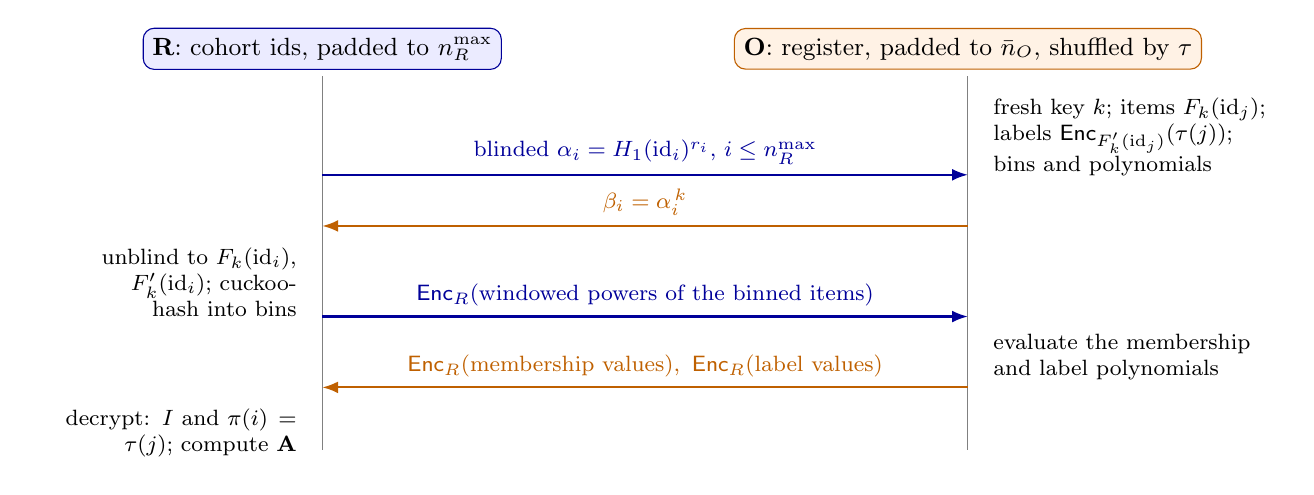
\begin{tikzpicture}[font=\small, >={Latex[length=2mm]}, every node/.style={align=center}]
  \def\xo{8.2}
  \node[fill=blue!8, draw=blue!60!black, rounded corners, minimum width=4.2cm] (R) at (0,0) {\textbf{R}: cohort ids, padded to $\nR$};
  \node[fill=orange!10, draw=orange!75!black, rounded corners, minimum width=4.6cm] (O) at (\xo,0) {\textbf{O}: register, padded to $\nO$, shuffled by $\tau$};
  \draw[gray] (0,-0.35) -- (0,-5.1); \draw[gray] (\xo,-0.35) -- (\xo,-5.1);
  \node[anchor=north west, font=\footnotesize, text width=3.6cm, align=left] at (\xo+0.2,-0.5) {fresh key $k$; items $F_k(\mathrm{id}_j)$; labels $\Enc_{F'_k(\mathrm{id}_j)}(\tau(j))$; bins and polynomials};
  \draw[->, blue!60!black, thick] (0,-1.6) -- node[above, font=\footnotesize] {blinded $\alpha_i=H_1(\mathrm{id}_i)^{r_i}$,\ $i\le\nR$} (\xo,-1.6);
  \draw[->, orange!75!black, thick] (\xo,-2.25) -- node[above, font=\footnotesize] {$\beta_i=\alpha_i^{\,k}$} (0,-2.25);
  \node[anchor=north east, font=\footnotesize, text width=3.3cm, align=right] at (-0.2,-2.4) {unblind to $F_k(\mathrm{id}_i)$, $F'_k(\mathrm{id}_i)$; cuckoo-hash into bins};
  \draw[->, blue!60!black, thick] (0,-3.4) -- node[above, font=\footnotesize] {$\Enc_R(\text{windowed powers of the binned items})$} (\xo,-3.4);
  \node[anchor=north west, font=\footnotesize, text width=3.6cm, align=left] at (\xo+0.2,-3.5) {evaluate the membership and label polynomials};
  \draw[->, orange!75!black, thick] (\xo,-4.3) -- node[above, font=\footnotesize] {$\Enc_R(\text{membership values}),\ \Enc_R(\text{label values})$} (0,-4.3);
  \node[anchor=north east, font=\footnotesize, text width=3.3cm, align=right] at (-0.2,-4.45) {decrypt: $I$ and $\pi(i)=\tau(j)$; compute $\mathbf A$};
\end{tikzpicture}
\caption{Phase 1 messages. Blue: $\Rp\to\Op$; orange: $\Op\to\Rp$. Everything $\Op$ receives is either a uniformly random group element or a ciphertext under $\Rp$'s own BFV key.}
\label{fig:flow}
\end{figure}

\begin{algorithm}[t]
\caption{Phase 1: link}\label{alg:link}
\begin{algorithmic}[1]
\Require $\Rp$: cohort identifiers $(\mathrm{id}_i)_{i\le n_R}$, $n_R\le\nR$. $\Op$: scope register $(\mathrm{id}_j,\mathbf x_{O,j},y_j)$. Public: $\nR$, $\nO$, PSI parameters.
\Ensure $\Rp$: match set $I$, positions $\pi(i)$ for $i\in I$, and its block $\mathbf A$. $\Op$: nothing.
\State \Odo pad the register with dummy rows to $\nO$; draw a fresh permutation $\tau$ of $[\nO]$ and a fresh OPRF key $k$
\State \Odo for each row $j$: item $F_k(\mathrm{id}_j)$, label $\Enc_{F'_k(\mathrm{id}_j)}(\tau(j))$; bin with three hash functions; pad bins and partitions to the public sizes; interpolate the membership and label polynomials
\State \Rdo pad the identifiers with random dummies to exactly $\nR$
\State \Rdo for each padded $\mathrm{id}_i$: send $\alpha_i=H_1(\mathrm{id}_i)^{r_i}$;\quad \Odo return $\beta_i=\alpha_i^{\,k}$ and log $\nR$ evaluations against the quota
\State \Rdo unblind to $F_k(\mathrm{id}_i)$ and $F'_k(\mathrm{id}_i)$; cuckoo-hash the items into the $m$ bins (dummies in empty bins)
\State \Rdo encrypt the binned items slot-wise under its own BFV key and send the windowed powers
\State \Odo evaluate the membership and label polynomials of every bin and partition; modulus-switch; reply
\State \Rdo decrypt; $i\in I$ iff some membership value of its bin is $0$; then $\pi(i)\gets$ the label value decrypted under $F'_k(\mathrm{id}_i)$
\State \Rdo $\mathbf A\gets\sum_{i\in I}\dot{\mathbf x}_i\dot{\mathbf x}_i^\top$ with $\dot{\mathbf x}_i=(1,\mathbf x_{R,i})$: exact and local
\end{algorithmic}
\end{algorithm}

\section{The protocol}

Figure~\ref{fig:flow} shows the messages and Algorithm~\ref{alg:link} the steps. The OPRF has two roles. It turns identifiers, often a small and guessable space such as social insurance numbers, into pseudorandom strings, so that the PSI messages carry no structure. And it makes every membership test an online interaction with $\Op$, so that $\Rp$ cannot test identifiers offline: $\Op$ evaluates exactly $\nR$ calls per run and logs them against a quota per researcher and project.

\paragraph{Worked example.} With the data of the companion worked-example deck: $\Rp$ holds identifiers $104$, $221$, $317$ and pads with one dummy, $9\mathrm{d}1$, to $\nR=4$. $\Op$ holds $088$, $104$, $150$, $221$, $399$, pads with $7\mathrm{e}5$ to $\nO=6$, and draws $\tau$:

\begin{center}\small
\begin{tabular}{@{}lcccccc@{}}
\toprule
$\Op$'s padded row $j$ & 150 & 7e5 (dummy) & 221 & 088 & 399 & 104 \\
position $\tau(j)$ & 1 & 2 & 3 & 4 & 5 & 6 \\
\bottomrule
\end{tabular}
\end{center}
$\Rp$ makes four OPRF calls. The PSI reply shows matches for $104$ and $221$, with decrypted labels $6$ and $3$, and no match for $317$ or the dummy. So $I=\{104,221\}$, $\pi(104)=6$ and $\pi(221)=3$. $\Op$ has seen four random group elements and a batch of ciphertexts it cannot decrypt.

\section{What each party learns}

\paragraph{$\Op$'s view.} The blinded elements $\alpha_i$ are uniform in the group, and the PSI query consists of ciphertexts under $\Rp$'s own key, which are pseudorandom under Ring-LWE. The number of OPRF calls and the query size depend only on $\nR$ and the public PSI parameters. $\Op$'s view can therefore be simulated from $(\nR,\nO)$: it learns neither the cohort, nor $n_R$, nor which of its rows match.

\paragraph{$\Rp$'s view.} $\Rp$ learns $F_k$ only at its own identifiers, so the PSI reply tells it nothing about register members it did not query. It learns membership of its padded identifiers, which is disclosed by design, and, for each match, a position that is uniform because $\tau$ is fresh. For a formal guarantee the replies must not leak $\Op$'s other items through their noise. Modulus switching reduces this leak, but the guarantee relies on circuit privacy of the BFV evaluation, for example by noise flooding; our proofs list this as an explicit assumption.

\paragraph{Limits.} The guarantee assumes $\Rp$ queries only its real cohort. A deviating $\Rp$ could use its $\nR$ calls to look up the membership of arbitrary people; the cap $\nR$, a certified cohort and the cross-session OPRF quota bound this. If membership itself is sensitive, circuit-PSI with payloads \cite{rs21} can give both parties secret shares of the alignment instead, at the price of a higher sensitivity in the release. Linkage is on exact identifiers only.

\paragraph{Correctness and cost.} The PSI parameters are chosen so that cuckoo hashing fails and false matches occur with probability at most $2^{-40}$; both affect correctness only and are not charged to the privacy budget. The OPRF costs two exponentiations per identifier for $\Rp$ and one for $\Op$. The PSI query depends only on $\nR$, and the reply grows with the number of partitions, which is sublinear in $\nO$ for suitable parameters. $\Op$'s preprocessing, however, is linear in $\nO$ and must be redone every run, because the key and the permutation are fresh. The public scope is therefore the main lever on cost. The phase takes two to three rounds.

\begin{thebibliography}{9}\small
\setlength{\itemsep}{0pt}
\bibitem{clr17} H.~Chen, K.~Laine, P.~Rindal. Fast private set intersection from homomorphic encryption. \emph{ACM CCS}, 2017.
\bibitem{chlr18} H.~Chen, Z.~Huang, K.~Laine, P.~Rindal. Labeled PSI from fully homomorphic encryption with malicious security. \emph{ACM CCS}, 2018.
\bibitem{cmg21} K.~Cong, R.~Cruz Moreno, M.~B.~da Gama, W.~Dai, I.~Iliashenko, K.~Laine, M.~Rosenberg. Labeled PSI from homomorphic encryption with reduced computation and communication. \emph{ACM CCS}, 2021.
\bibitem{jkk14} S.~Jarecki, A.~Kiayias, H.~Krawczyk. Round-optimal password-protected secret sharing and T-PAKE in the password-only model. \emph{ASIACRYPT}, 2014.
\bibitem{rfc9497} A.~Davidson, A.~Faz-Hern\'andez, N.~Sullivan, C.~A.~Wood. Oblivious pseudorandom functions (OPRFs) using prime-order groups. RFC~9497, 2023.
\bibitem{rs21} P.~Rindal, P.~Schoppmann. VOLE-PSI: fast OPRF and circuit-PSI from vector-OLE. \emph{EUROCRYPT}, 2021.
\bibitem{pr04} R.~Pagh, F.~F.~Rodler. Cuckoo hashing. \emph{Journal of Algorithms} 51(2), 2004.
\end{thebibliography}

\end{document}
